\documentclass[xcolor=pdftex,table,10pt]{beamer}

\usetheme{UBS}  

\usepackage[default,scale=0.95]{opensans}
\usepackage[french]{babel}
\usepackage[utf8]{inputenc}
\usepackage{fancybox}
\usepackage{amsmath}
\usepackage{amsfonts}
\usepackage{color}
\usepackage{tabularx}
\usepackage{graphicx}
\usepackage{enumerate}
\usepackage{multirow}
\usepackage{wasysym}
%\usepackage{slashbox}
\usepackage{hhline}
\usepackage{eurosym}
\usepackage{subfigure}
\usepackage{colortbl}
\usepackage{booktabs}
\usepackage[percent]{overpic}
\usepackage{tikz}
\usetikzlibrary{automata,trees,calc,shadings,shapes.gates.logic.US,positioning,arrows}

%\newcommand<>{\btikzset}[2]{\alt#3{\tikzset{#1}}{\tikzset{#2}}}
%\renewcommand<>{\tikzset}[1]{\only#2{\beameroriginal{\tikzset}{#1}}}

%\tikzset{hide on/.code={\only<#1>{\color{fg!20}}}}

\tikzset{
  invisible/.style={opacity=0,text opacity=0},
  visible on/.style={alt={#1{}{invisible}}},
  alt/.code args={<#1>#2#3}{%
    \alt<#1>{\pgfkeysalso{#2}}{\pgfkeysalso{#3}} % \pgfkeysalso doesn't change the path
  },
}


\tikzset{onslide/.code args={<#1>#2}{%
  \only<#1>{\pgfkeysalso{#2}} % \pgfkeysalso doesn't change the path
}}
% \tikzset{temporal/.code args={<#1>#2#3#4}{%
%   \temporal<#1>{\pgfkeysalso{#2}}{\pgfkeysalso{#3}}{\pgfkeysalso{#4}} % \pgfkeysalso doesn't change the path
% }}

% \tikzstyle{highlight}=[red,ultra thick]

\usepackage[style=authoryear,isbn=false,doi=false,url=false]{biblatex}
\bibliography{../../biblio/biblio_libre}
\renewcommand{\bibfont}{\normalfont\tiny}

% EdgeMind Colors
\definecolor{EMLogoBlue}        {cmyk}{0.96, 0.75, 0.30, 0.18} 
%\definecolor{EMLogoOrange}      {cmyk}{0.00, 0.61, 0.90, 0.00} 

%\definecolor{EMGrey}            {cmyk}{0.21, 0.17, 0.10, 0.00} 
%\definecolor{EMBrownLight}      {cmyk}{0.25, 0.47, 0.75, 0.15} 
%\definecolor{EMRed}             {cmyk}{0.21, 1.00, 0.92, 0.14} 
%\definecolor{EMBrown}           {cmyk}{0.34, 1.00, 0.91, 0.55} 

%\everymath\expandafter{\the\everymath \color{EMLogoBlue}}
%\everydisplay\expandafter{\the\everydisplay \color{EMLogoBlue}}


%\newtheorem{remarks}{Remarks}

% Math fonts
% ----------
%\usepackage{euler} 
%\usepackage{mathptm}
%\usepackage{mathrsfs}
%\usepackage{mathpple}

% In order to do bold caligraphy math
\DeclareSymbolFont{boldsymbols}{OMS}{cmsy}{b}{n}
\DeclareSymbolFontAlphabet{\mathbfcal}{boldsymbols}


% \def\Then{\Rightarrow}
\usepackage{macros_math_rd}

%\usepackage[french,ruled,lined]{algorithm2e}

\usepackage{algorithm}
\usepackage{algorithmic}
\renewcommand{\algorithmicrequire}{\textbf{Entrée:}}
\renewcommand{\algorithmicensure}{\textbf{Sortie:}}
\renewcommand{\algorithmiccomment}[1]{\{#1\}}
\renewcommand{\algorithmicend}{\textbf{Fin}}
\renewcommand{\algorithmicif}{\textbf{Si}}
\renewcommand{\algorithmicthen}{\textbf{Alors}}
\renewcommand{\algorithmicelse}{\textbf{Sinon}}
\renewcommand{\algorithmicelsif}{\algorithmicelse\ \algorithmicif}
\renewcommand{\algorithmicendif}{\algorithmicend\ \algorithmicif}
\renewcommand{\algorithmicfor}{\textbf{Pour}}
\renewcommand{\algorithmicforall}{\textbf{Pour chaque}}
\renewcommand{\algorithmicdo}{\textbf{Faire}}
\renewcommand{\algorithmicendfor}{\algorithmicend\ \algorithmicfor}
\renewcommand{\algorithmicwhile}{\textbf{Tant que}}


% Graphics path
% -------------
\graphicspath{ 
  {./fig/}
}




% =============
% =============

% Title, author, date
\title{Modélisation Stochastique et Réseaux Bayésiens}
\subtitle{Apprentissage automatique des lois de probabilité conditionnelles}

\date[ENSIBS - Spécialité informatique]{
  ENSIBS - Spécialité informatique \\[0.5cm]
  
  {\color{EMLogoBlue}\scriptsize{\url{http://www.edgemind.net/teaching/ensibs/mod-stoch-rb/}}}
}

\author[Roland Donat]{Roland Donat}

\institute[UBS]{Université de Bretagne Sud}

\AtBeginSection[]
{
\begin{frame}<beamer>
\frametitle{Plan}
\tableofcontents[currentsection, hideothersubsections]
\end{frame}
}


% ============================
% ============================

\begin{document}

% Title
\begin{frame}[plain]
    \titlepage
\end{frame}

%\setbeamertemplate{background canvas}{\pgfuseimage{fond_slide}}



\frame{
  \frametitle{Plan de la présentation}
  \tableofcontents[sectionstyle=show/show,subsectionstyle=hide/hide/hide]
}



\frame{
  \frametitle{Objectifs pédagogiques}
  \begin{itemize}
  \item Comprendre les problématiques liées à la construction pratique d'un réseau bayésien
  \item Prendre connaissance des approches de construction de RB à partir de jugements d'experts
  \item Savoir construire un RB automatiquement à partir d'un jeu de données
  \end{itemize}
}



\section[Intro]{Introduction}

\frame{
\frametitle{Introduction}
\framesubtitle{Objectif}

\begin{block}{Objectif}
\begin{itemize}
\item Modéliser un phénomène aléatoire à partir d'un RB 
\itemThenC Représenter la loi jointe d'une suite de v.a. $\mbf{X} =
\lrpar{X_{1}, \ldots, X_{D}}$
\end{itemize}
\end{block}

\pause

\begin{block}{Problèmes}
\begin{itemize}
\item Comment déterminer la structure du RB (i.e. le graphe)?
\item Comment estimer les lois de probabilité conditionnelles (LPC) :
$
\Prob\lrPar{X_{d}|\pa\lrPar{X_{d}}},~ d = 1, \ldots, D
$?
\end{itemize}
\end{block}

\pause

\begin{exampleblock}{Approches envisageables}
\begin{itemize}
\item Approche par expertise : Utilisation d'avis d'experts et connaissances métiers
\item Approche statistique : Utilisation de bases de données (contenant éventuellement des
  informations incomplètes)
\item Approche mixte : expertise + bases de données
\end{itemize}
\end{exampleblock}
}

\frame{
\frametitle{Introduction}
\framesubtitle{Exemple : Pourquoi l'herbe de mon jardin est-elle mouillée?}

% \begin{columns}
%   \column{0.45\textwidth}{
    \begin{center}
      \begin{overlayarea}{\textwidth}{\textheight}
        \only<2>{\includegraphics[width=\textwidth]{rb_sprinkler_fr_v2_var.pdf}}
        \only<3>{\includegraphics[width=\textwidth]{rb_sprinkler_fr_v2_dag.pdf}}
        \only<4>{\includegraphics[width=\textwidth]{rb_sprinkler_fr_v2_lpc.pdf}}
        \only<5>{\includegraphics[width=\textwidth]{rb_sprinkler_fr_v2_learning.pdf}}
      \end{overlayarea}
    \end{center}
%   }
%   % A l'époque tous ceux qui font des probas utilisent un vocabulaire lié aux jeux d'argent (paris, côte etc...)
%   \column{0.45\textwidth}{
%     \begin{exampleblock}{Exemples de requêtes}
%       \begin{itemize}
%         \item<2-> $\Prob\lrPar{{\color{EMLogoOrange}{X_{6}}}}$
%         \item<3-> $\Prob\lrPar{{\color{EMLogoOrange}{X_{4}}}}$
%         \item<4-> $\Prob\lrPar{{\color{EMLogoOrange}{X_{4}}}|{\color{EMLogoBlue}{X_{5} =
%                   x_{5}}}}$
%         \item<5-> $\Prob\lrPar{{\color{EMLogoOrange}{X_{2}}}|{\color{EMLogoBlue}{X_{1} =
%                   x_{1},X_{6} = x_{6}}}}$
%         \item<6-> $\Prob\lrPar{{\color{EMLogoOrange}{X_{3}, X_{5}}}|{\color{EMLogoBlue}{X_{4} =
%                   x_{4},X_{6} = x_{6}}}}$
%       \end{itemize}
%     \end{exampleblock}
%   }
% \end{columns}
}


\section[App. experts]{Construction d'un RB par jugements d'experts}

\subsection{Acquisition de l'information}

\frame{
\frametitle{Construction d'un RB par jugements d'experts}
\framesubtitle{Acquisition de l'information}

\begin{block}{Acquisition de l'information}
\begin{itemize}
\item Trouver un ou plusieurs experts fiables et coopératifs
\item Les familiariser à la notion de probabilité
\item Tenir compte des biais éventuels parfois subconscients (un expert va souvent sur-estimer la
  probabilité de réussite d’un projet le concernant, etc.)
\item Lui fournir un outil pour déterminer les probabilités
\begin{itemize}
\itemThenC<2-> Exemple : échelle de probabilité
\end{itemize}
\end{itemize}
\end{block}

  \begin{overlayarea}{\textwidth}{\textheight}
\begin{center}
    \only<2->{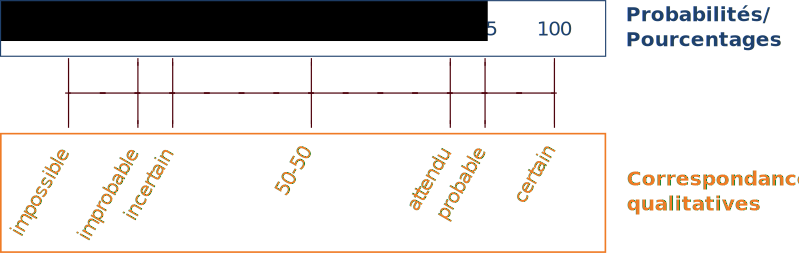
\includegraphics[width=0.8\textwidth]{echelle_prob.pdf}}
\end{center}
  \end{overlayarea}

}

\subsection{Simplification des LPC : Modèle OU-bruité}

\frame{
\frametitle{Construction d'un RB par jugements d'experts}
\framesubtitle{Attention au connexions convergentes (V-structures)}

\begin{block}{Problème}
\begin{itemize}
\item L'expertise métier permet en général de construire des RB fidèles à la réalité opérationnelle
\item En revanche, l'humaine a intuitivement tendance à introduire des connexions convergentes
\begin{itemize}
\item Exemple : Soit $Y$ un phénomène à expliquer et $X_{1}, \ldots, X_{n}$, $n$ facteurs possibles
\item Structure naturelle : $X_{1}, \ldots, X_{n} \to Y$
\end{itemize}
\itemThenC Risque d'explosion combinatoire
\end{itemize}
\end{block}

\pause

\begin{exampleblock}{Solution possible : Simplifier la LPC des structures convergentes} 
\begin{itemize}
\item Exemple : Traitement des LPC du type $\Prob\lrPar{Y|X_{1},\ldots,X_{n}}$ où les v.a. sont binaires
\itemThenC Dans le cas général, définir $\Prob\lrPar{Y|X_{1},\ldots,X_{n}}$ nécessite \alert{$2^{n}$
  valeurs!}
\itemThenC Introduction d'un modèle de LPC particulier : modèle OU-bruité
\end{itemize}
\end{exampleblock}

}


\frame{
\frametitle{Construction d'un RB par jugements d'experts}
\framesubtitle{Simplification des LPC : Modèle OU-bruité}

\begin{block}{Formulation du modèle OU-bruité (\textit{Noisy-OR}, \cite{Pearl1986Fusion})}
\begin{itemize}
\item Hypothèse 1 : Il est possible d'estimer les probabilités $p_{i} = \Prob\lrPar{Y = y|X_{1} = \bar{x}_{1},
    \ldots, X_{i} = x_{i}, \ldots, X_{n} = \bar{x}_{n}}$ (e.g. par avis experts)
\item Hypothèse 2 : Les v.a. $X_{i}$ influent sur $Y$ de manière indépendante
\itemThenC Si $X_{i}$ seule est à "vrai", alors $Y$ est à "vrai" avec la
  probabilité $p_{i}$
\itemThenC Si plusieurs $X_{i}$ sont à "vrai", alors :
$$
\Prob\lrPar{Y = y|\mbf{X}_{\text{vrai}} = \mbf{x}, \mbf{X}_{\text{faux}} = \bar{\mbf{x}}} = 1 -
\prod_{i | X_{i} \in \mbf{X}_{\text{vrai}}} (1 - p_{i})
$$
où $\mbf{X}_{\text{vrai/faux}}$ est la suite de v.a. à "vrai"/"faux" avec
$\lrPar{X_{1},\ldots,X_{n}} = \mbf{X}_{\text{vrai}} \union \mbf{X}_{\text{faux}}$
\end{itemize}
\end{block}

}


\frame{
\frametitle{Construction d'un RB par jugements d'experts}
\framesubtitle{Modèle OU-bruité - Illustration}

\begin{overlayarea}{\textwidth}{0.33\textheight}
\begin{center}
  \only<1->{\includegraphics[width=0.66\textwidth]{rb_fievre.pdf}}
\end{center}
\end{overlayarea}
\begin{overlayarea}{\textwidth}{0.75\textheight}
  \begin{center}
    \only<2>{\includegraphics[width=0.75\textwidth]{rb_fievre_lpc_noisy_or_vide.pdf}}
    \only<3>{\includegraphics[width=0.75\textwidth]{rb_fievre_lpc_noisy_or_hyp_tt_faux.pdf}}
    \only<4>{\includegraphics[width=0.75\textwidth]{rb_fievre_lpc_noisy_or_hyp_pi.pdf}}
    \only<5>{\includegraphics[width=0.75\textwidth]{rb_fievre_lpc_noisy_or_1.pdf}}
    \only<6>{\includegraphics[width=0.75\textwidth]{rb_fievre_lpc_noisy_or_2.pdf}}
    \only<7>{\includegraphics[width=0.75\textwidth]{rb_fievre_lpc_noisy_or_3.pdf}}
    \only<8>{\includegraphics[width=0.75\textwidth]{rb_fievre_lpc_noisy_or_4.pdf}}
    \only<9>{\includegraphics[width=0.75\textwidth]{rb_fievre_lpc_noisy_or.pdf}}
  \end{center}
\end{overlayarea}

}


\frame{
\frametitle{Construction d'un RB par jugements d'experts}
\framesubtitle{Modèle OU-bruité - Remarques et extensions}


\begin{exampleblock}{Remarques}
\begin{itemize}
\item Le modèle OU-bruité est une généralisation aléatoire du OU logique
\item Ce modèle de LPC s'intègre bien aux algorithmes d'inférence exacte
\item Ce modèle peut également être utilisé pour l'apprentissage de LPC à partir de données
\end{itemize}
\end{exampleblock}

\pause

\begin{block}{Extensions du modèle OU-bruité}
\begin{itemize}
\item \textit{Leaky Noisy-OR} : $Y$ peut être vrai sans cause $X_{i}$ vraie
  \parencite{Henrion1988Practical}
\item Généralisation au cas où les variables $X_{i}$ ne sont plus binaires \parencite{Srinivas1993NoisyOr, Pradhan_al1994Knowledge}
\end{itemize}
\end{block}

}

\section[Rappels stat]{Rappels statistiques}

\frame{
\frametitle{Rappels statistiques}
\framesubtitle{Base de données - Définition}

\begin{block}{Définition : Base de données}
\begin{itemize}
\item Une base de données (BdD), notée $\mathcal{D}$, est un ensemble de $N$ individus/observations/exemples
  caractérisés par $D$ variables
\item Formellement, une BdD peut se mettre sous la forme d'une matrice :
\begin{equation*}
\mathcal{D} = 
\lrBrack{
\begin{array}{ccccc}
x_{1,1} & \ldots & x_{1,d} & \ldots & x_{1,D} \\
\vdots  &        & \vdots  &        & \vdots \\
x_{n,1} & \ldots & x_{n,d} & \ldots & x_{n,D} \\
\vdots  &        & \vdots  &        & \vdots \\  
x_{N,1} & \ldots & x_{N,d} & \ldots & x_{N,D} \\
\end{array}
}
\end{equation*}
\begin{itemize}
\item Le vecteur colonne $\mbf{x}_{\cdot, d} = \lrPar{x_{1,d}, \ldots, x_{n,d}, \ldots, x_{N,d}}$ représente toutes les observations de la variable $d$
\item Le vecteur ligne $\mbf{x}_{n, \cdot} = \lrPar{x_{n,1}, \ldots, x_{n,d}, \ldots, x_{n,D}}$ représente le $n$-ème individu de la BdD
\end{itemize}
\end{itemize}
\end{block}

}

\frame{
\frametitle{Rappels statistiques}
\framesubtitle{Base de données - Exemple}

\begin{columns}
  \column{0.5\textwidth}{
    \begin{center}
      \begin{overlayarea}{\textwidth}{0.75\textheight}
        \only<1>{\includegraphics[width=\textwidth]{donnees_5_var.pdf}}
        \only<2>{\includegraphics[width=\textwidth]{donnees_5_var_hi_var.pdf}}
        \only<3>{\includegraphics[width=\textwidth]{donnees_5_var_hi_col.pdf}}
        \only<4>{\includegraphics[width=\textwidth]{donnees_5_var_hi_line.pdf}}
      \end{overlayarea}
    \end{center}
  }
  \column{0.45\textwidth}{
    \only<2->{    
    \begin{exampleblock}{Caractéristiques des données}
      \begin{itemize}
      \item<2-> Nombre de variables : 5
      \item<3-> Observations de la variable "FT"
      \item<4-> Individu caractérisé par le vecteur (2013-08-10, Lille, Lorient, 1-0, 1-0)
      \end{itemize}
    \end{exampleblock}
    }
  }
\end{columns}
}


\frame{
\frametitle{Rappels statistiques}
\framesubtitle{Modélisation statistique : objectifs et démarche}

\begin{block}{Objectifs}
\begin{enumerate}
\item Résumer quantitativement l'information contenue dans une BdD en utilisant un modèle probabiliste
\item Exploiter le modèle pour déduire de nouvelles connaissances
\end{enumerate}
\end{block}

\pause

\begin{block}{Démarche}
\begin{itemize}
\item Considérer les données comme des réalisations de variables aléatoires (v.a.) associées à une
  certaine loi jointe
\item Formellement, cela signifie que chaque observation $\mbf{x}_{n, \cdot} = \lrPar{x_{n,1}, \ldots,
    x_{n,D}}$ est supposée être une réalisation d'une suite de v.a. $\mbf{X} =
  \lrPar{X_{1},\ldots,X_{D}}$ de loi jointe
  $\mathcal{L}\lrPar{\mbf{\theta}}$ où $\mbf{\theta}$ représente les paramètres de la loi
\item Notation : $\mbf{X} = \lrPar{X_{1},\ldots,X_{D}} \sim \mathcal{L}\lrPar{\mbf{\theta}}$
\end{itemize}
\end{block}

}


\frame{
\frametitle{Rappels statistiques}
\framesubtitle{Modélisation statistique : remarques et exemple}

\begin{block}{Remarques}
\begin{itemize}
\item Si les individus dans les données sont indépendants, on parle de données i.i.d. (Indépendantes et
  Identiquement Distribuées)
\item Si les caractéristiques des individus (variables) sont indépendantes, alors chaque variable
  $X_{d}$ suit une loi $\mathcal{L}_{d}\lrpar{\mbf{\theta}_{d}}$ (Notation : $X_{d} \sim \mathcal{L}_{d}\lrpar{\mbf{\theta}_{d}}$)
\end{itemize}
\end{block}

\pause

\begin{exampleblock}{Modèle gaussien}
\begin{itemize}
\item Données unidimensionnelles ($D = 1$)
\itemThenC $\mbf{X} = X_{1} \sim \mathcal{N}\lrPar{\mu, \sigma}$
\itemThenC $\mbf{\theta} = (\mu,\sigma)$ : moyenne et écart-type
\item Données multidimensionnelles ($D \ge 1$)
\itemThenC $\mbf{X} = \lrPar{X_{1},\ldots,X_{D}} \sim \mathcal{N}\lrPar{\mbf{\mu}, \mbf{\Sigma}}$
\itemThenC $\mbf{\theta} = (\mbf{\mu},\mbf{\Sigma})$ : vecteur des moyennes et matrice de variance-covariance
\end{itemize}
\end{exampleblock}

}


\frame{
\frametitle{Rappels statistiques}
\framesubtitle{Estimation des paramètres d'un modèle}

\begin{block}{Contexte}
\begin{itemize}
\item Données : On dispose d'un jeu de données $\mathcal{D} = \lrpar{\mbf{x}_{1,\cdot}, \ldots, \mbf{x}_{N,\cdot}}$
  où chaque observation $\mbf{x}_{n,\cdot}$ est caractérisée par $D$ variables $\lrPar{x_{n,1},\ldots,x_{n,D}}$ 
\item Modélisation : On suppose que $\mathcal{D}$ est une suite de $N$ réalisations i.i.d. du vecteur aléatoire
  $\mbf{X} = \lrpar{X_{1}, \ldots, X_{D}}$ distribué selon la loi $\mathcal{L}\lrPar{\mbf{\theta}}$ 
\item \alert{Problématique : Comment estimer les paramètres $\mbf{\theta}$ à partir des données
    $\mathcal{D}$?}
\end{itemize}
\end{block}

\pause

\begin{block}{Solution}
\begin{itemize}
\item Construire un estimateur de $\mbf{\theta}$!
\itemThenC Approche classique : Déterminer l'estimateur du maximum de vraisemblance de
$\mbf{\theta}$, souvent noté $\mbf{\theta}^{\text{MV}}$
\end{itemize}
\end{block}

}


\frame{
\frametitle{Rappels statistiques}
\framesubtitle{Définition de la vraisemblance d'un individu}

\begin{block}{Vraisemblance d'un individu}
\begin{itemize}
\item Soit $\mathcal{D} = \lrpar{\mbf{x}_{1,\cdot}, \ldots, \mbf{x}_{N,\cdot}}$ un ensemble de
  données i.i.d. modélisées par les v.a. $\mbf{X} = \lrpar{X_{1}, \ldots, X_{D}} \sim \mathcal{L}\lrPar{\mbf{\theta}}$ 
\item La vraisemblance d'un individu $\mbf{x}_{n,\cdot} \in \mathcal{D}$ dans le modèle probabiliste
  choisi (paramétré par $\mbf{\theta}$) est notée $L\lrPar{\mbf{\theta};\mbf{x}_{n,\cdot}}$
\item La vraisemblance $L\lrPar{\mbf{\theta};\mbf{x}_{n,\cdot}}$ correspond
  simplement à la probabilité d'observer $\mbf{x}_{n,\cdot}$  dans le modèle
  $\mathcal{L}\lrPar{\mbf{\theta}}$
\item En pratique le logarithme de la vraisemblance est souvent utilisé, on parle alors de
  log-vraisemblance $\ell\lrPar{\mbf{\theta};\mbf{x}_{n,\cdot}} = \ln L\lrPar{\mbf{\theta};\mbf{x}_{n,\cdot}}$
\end{itemize}
\end{block}

\pause

\begin{block}{Interprétation}
  En considérant un modèle probabiliste donné et un individu :
\begin{itemize}
\item une vraisemblance \textbf{élevée (i.e. proche de 1)} signifie que
  le modèle prévoit \textbf{l'observation fréquente} de ce type d'individus
\item une vraisemblance \textbf{faible (i.e. proche de 0)} signifie que
  le modèle prévoit de \textbf{rares observations} de ce type d'individus
\end{itemize}
\end{block}

}

\frame{
\frametitle{Rappels statistiques}
\framesubtitle{Vraisemblance d'un individu discret et fini}

\begin{block}{Vraisemblance d'un individu discret et fini}
\begin{itemize}
\item Si les v.a. $\mbf{X} = \lrpar{X_{1}, \ldots, X_{D}}$ sont discrètes et finies, alors 
$$
L\lrPar{\mbf{\theta};\mbf{x}_{n,\cdot}} = \Prob\lrPar{X_{1} = x_{n,1},\ldots, X_{D} = x_{n,D}; \mbf{\theta}}
$$
\item $\mbf{\theta}$ correspond au vecteur de probabilités de la loi jointe des v.a.
\end{itemize}
\end{block}

\begin{exampleblock}{Exemple}
\begin{columns}
  \column{0.5\textwidth}{
\begin{overlayarea}{\textwidth}{0.5\textheight}
  %% \begin{center}
  %%   \only<2->{\color{EMLogoBlue}\textbf{Modélisation : Loi jointe}}
  %% \end{center}
  \begin{center}
    \only<2>{\includegraphics[width=0.6\textwidth]{rb_bank_marketing_3_var_loi_jointe.pdf}}
    \only<3->{\includegraphics[width=0.6\textwidth]{rb_bank_marketing_3_var_loi_jointe_hi_indiv.pdf}}
  \end{center}
\end{overlayarea}
  }
  \column{0.5\textwidth}{
    \begin{itemize}
    \item<3-> Individu caractérisé par
      \begin{itemize}
      \item<3-> Âge : [26,59]
      \item<3-> Épargne : non
      \item<3-> Vente livret A : échec
      \end{itemize}
      \itemThenC<4-> Vraisemblance = 0.12
      \itemThenC<4-> Log-vraisemblance $\simeq$ 2.12
    \end{itemize}
  }
\end{columns}
\end{exampleblock}

}


\frame{
\frametitle{Rappels statistiques}
\framesubtitle{Vraisemblance d'un jeu de données}

\begin{block}{Vraisemblance d'un jeu de données}
\begin{itemize}
% \item Soit $\mathcal{D} = \lrpar{\mbf{x}_{1,\cdot}, \ldots, \mbf{x}_{N,\cdot}}$ un ensemble de
%   données i.i.d. modélisées par les v.a. $\mbf{X} = \lrpar{X_{1}, \ldots, X_{D}} \sim \mathcal{L}\lrPar{\mbf{\theta}}$ 
\item La vraisemblance d'un jeu de données $\mathcal{D}$
  dans le modèle probabiliste choisi
  (paramétré par $\mbf{\theta}$) est notée $L\lrPar{\mbf{\theta};\mathcal{D}}$
\item La vraisemblance $L\lrPar{\mbf{\theta};\mathcal{D}}$ correspond
  à la probabilité d'observer les données $\mathcal{D}$ dans ce modèle
\item Lorsque les données sont supposées i.i.d., la vraisemblance de $\mathcal{D}$ est définie par 
$$
L\lrPar{\mbf{\theta};\mathcal{D}} = \prod_{n = 1}^{N} L\lrPar{\mbf{\theta};\mbf{x}_{n,\cdot}}
$$
\item En pratique, la log-vraisemblance est toujours utilisée lorsque l'on s'intéresse à un jeu de
  données. La log-vraisemblance est définie par
  $$
\ell\lrPar{\mbf{\theta};\mathcal{D}} = \ln L\lrPar{\mbf{\theta};\mathcal{D}} = \sum_{n = 1}^{N} \ell\lrPar{\mbf{\theta};\mbf{x}_{n,\cdot}}
$$

\end{itemize}
\end{block}

}


\frame{
\frametitle{Rappels statistiques}
\framesubtitle{Vraisemblance d'un jeu de données}

\begin{block}{Interprétation}
  \begin{itemize}
  \item La vraisemblance est une fonction prenant comme argument un modèle probabiliste caractérisé
    par ses paramètres $\mbf{\theta}$ et retournant un réel
  \item La vraisemblance est indicateur permettant de comparer différents modèles probabilistes pour
    un jeu de données fixé
\item Dans l'absolu plus la log-vraisemblance d'un jeu de données $\mathcal{D}$ est élevée, plus le
  modèle probabiliste considéré est adapté aux données observées
  \end{itemize}
\end{block}

\begin{alertblock}{Attention}
  \begin{itemize}
  \item La vraisemblance d'un jeu de données dans un modèle probabiliste décroît avec le nombre de données observé
  \itemThenC Il n'est pas pertinent de comparer des vraisemblances obtenues à partir de jeux de
  données de taille différente
  \itemThenC En revanche, il peut être intéressant de comparer des vraisemblances moyennes par
  donnée observée
  \end{itemize}
\end{alertblock}
  
}


\frame{
\frametitle{Rappels statistiques}
\framesubtitle{Vraisemblance d'un jeu de données - Exemple}

\begin{columns}
  \column{0.5\textwidth}{
\begin{overlayarea}{\textwidth}{0.75\textheight}
  \begin{center}
    \only<1->{\color{EMLogoBlue}\textbf{Loi jointe}}
  \end{center}
  \begin{center}
    \only<1>{\includegraphics[width=1.0\textwidth]{rb_bank_marketing_3_var_loi_jointe.pdf}}
    \only<2>{\includegraphics[width=1.0\textwidth]{rb_bank_marketing_3_var_loi_jointe_hi_indiv.pdf}}
    \only<3>{\includegraphics[width=1.0\textwidth]{rb_bank_marketing_3_var_loi_jointe_hi_indiv_2.pdf}}
    \only<4>{\includegraphics[width=1.0\textwidth]{rb_bank_marketing_3_var_loi_jointe_hi_indiv_3.pdf}}
    \only<5->{\includegraphics[width=1.0\textwidth]{rb_bank_marketing_3_var_loi_jointe.pdf}}
  \end{center}
\end{overlayarea}
  }
  \column{0.5\textwidth}{
    \begin{overlayarea}{\textwidth}{0.725\textheight}
      \begin{center}
        \only<1->{\color{EMLogoBlue}\textbf{Données}}
      \end{center}
      \begin{center}
        \only<1>{\includegraphics[width=1.0\textwidth]{data_bank_marketing_3_var_3_data.pdf}}
        \only<2>{\includegraphics[width=1.0\textwidth]{data_bank_marketing_3_var_3_data_L1.pdf}}
        \only<3>{\includegraphics[width=1.0\textwidth]{data_bank_marketing_3_var_3_data_L2.pdf}}
        \only<4>{\includegraphics[width=1.0\textwidth]{data_bank_marketing_3_var_3_data_L3.pdf}}
        \only<5>{\includegraphics[width=1.0\textwidth]{data_bank_marketing_3_var_3_data_Ltot.pdf}}

      \end{center}
    \end{overlayarea}
  }
\end{columns}

}


\frame{
\frametitle{Rappels statistiques}
\framesubtitle{Estimateur du maximum de vraisemblance}

\begin{block}{Estimateur du maximum de vraisemblance \parencite{Fisher1922TheoreticalStatistics}}
\begin{itemize}
\item Soit $\mathcal{D} = \lrpar{\mbf{x}_{1,\cdot}, \ldots, \mbf{x}_{N,\cdot}}$ un ensemble de
  données supposées i.i.d. modélisées par les v.a. $\mbf{X} = \lrpar{X_{1}, \ldots, X_{D}} \sim \mathcal{L}\lrPar{\mbf{\theta}}$ 
\item On dit que $\mbf{\theta}^{\text{MV}}$ est un estimateur du maximum de vraisemblance (EMV) de
  $\mbf{\theta}$ si $\mbf{\theta}^{\text{MV}}$ maximise la vraisemblance des données, c-à-d. 
  $$
  \mbf{\theta}^{\text{MV}} = \argmax{\mbf{\theta}} L\lrPar{\mbf{\theta};\mathcal{D}}
  $$
\end{itemize}
\end{block}

\pause

\begin{block}{Propriétés des EMV}
Les EMV sont :
\begin{itemize}
\item Convergents en probabilité vers les paramètres à estimer
\item Efficaces, i.e. ils convergent rapidement
\item Asymptotiquement normaux, i.e. il est facile de construire des intervalles de
  confiance sur les estimations obtenues
\end{itemize}
\end{block}

}


\section[LPC - données complètes]{Apprentissage des LPC : Données complètes}

\subsection{Contexte}

\frame{
\frametitle{Apprentissage des LPC : Données complètes}
\framesubtitle{Contexte}

\begin{block}{Contexte}
\begin{itemize}
\item Données : On dispose d'un jeu de données $\mathcal{D} = \lrpar{\mbf{x}_{1,\cdot}, \ldots, \mbf{x}_{N,\cdot}}$
  où chaque observation $\mbf{x}_{n,\cdot}$ est caractérisée par $D$ variables $\lrPar{x_{n,1},\ldots,x_{n,D}}$ 
\item Modélisation : On suppose que $\mathcal{D}$ est une suite de $N$ réalisations i.i.d. du
  vecteur aléatoire discret et fini $\mbf{X} = \lrpar{X_{1}, \ldots, X_{D}}$ représenté par un RB $\mathcal{M}$
  défini par ses LPC $\theta_{d} = \lrPar{\Prob\lrPar{X_{d}|\pa\lrPar{X_{d}}}}_{d = 1,\ldots, D}$
\item Le graphe du RB est supposé connu
\end{itemize}
\end{block}

}


\frame{
\frametitle{Apprentissage des LPC : Données complètes}
\framesubtitle{Contexte - Exemple}

\begin{columns}
  \column{0.5\textwidth}{
\begin{overlayarea}{\textwidth}{0.75\textheight}
  \begin{center}
    \only<1->{\color{EMLogoBlue}\textbf{Données}}
  \end{center}
  \begin{center}
    \only<1->{\includegraphics[width=0.9\textwidth]{data_bank_marketing_3_var.pdf}}
  \end{center}
\end{overlayarea}
  }
  \column{0.5\textwidth}{
      \begin{overlayarea}{\textwidth}{0.725\textheight}
    \begin{center}
      \only<2->{\color{EMLogoBlue}\textbf{Modélisation}}
    \end{center}
    \begin{center}
      \only<2->{\includegraphics[width=\textwidth]{rb_bank_marketing_3_var.pdf}}
    \end{center}
  \end{overlayarea}
  }
\end{columns}

}


\subsection{Vraisemblance dans un RB}


\frame{
\frametitle{Apprentissage des LPC : Données complètes}
\framesubtitle{Vraisemblance dans un RB}

\begin{block}{Vraisemblance dans un RB}
\begin{itemize}
\item La vraisemblance d'une donnée $\mbf{x}_{n,\cdot} \in \mathcal{D}$ dans le RB
  $\mathcal{M}\lrPar{\theta_{1},\ldots,\theta_{D}}$ est définie par
  \begin{align*}
    L\lrPar{\theta_{1},\ldots,\theta_{D};\mbf{x}_{n,\cdot}} = & \prod_{d = 1}^{D} \Prob\lrPar{X_{d}
      = x_{n,d}|\pa\lrPar{X_{d}} = \pa\lrPar{x_{n,d}}} 
  \end{align*}
\itemThenC La vraisemblance des données $\mathcal{D}$ i.i.d. dans le RB
  $\mathcal{M}\lrPar{\theta_{1},\ldots,\theta_{D}}$ est définie par
  \begin{align*}
    L\lrPar{\theta_{1},\ldots,\theta_{D};\mathcal{D}} = & \prod_{n = 1}^{N} \prod_{d = 1}^{D} \Prob\lrPar{X_{d}
      = x_{n,d}|\pa\lrPar{X_{d}} = \pa\lrPar{x_{n,d}}} 
  \end{align*}
  \itemThenC On en déduit la log-vraisemblance :
  \begin{align*}
    \ell\lrPar{\theta_{1},\ldots,\theta_{D};\mathcal{D}} = & \sum_{n = 1}^{N} \sum_{d = 1}^{D} \ln \Prob\lrPar{X_{d}
      = x_{n,d}|\pa\lrPar{X_{d}} = \pa\lrPar{x_{n,d}}} 
  \end{align*}

\end{itemize}
\end{block}


}


\subsection{EMV dans un RB}

\frame{
\frametitle{Apprentissage des LPC : Données complètes}
\framesubtitle{Maximum de vraisemblance dans un RB}

\begin{block}{Estimateurs du maximum de vraisemblance}
\begin{itemize}
\item On cherche les estimateurs du maximum de vraisemblance (EMV) des LPC $\theta^{\text{MV}}_{1},\ldots, \theta^{\text{MV}}_{D}$
  vérifiant :
  $$
  \lrPar{\theta^{\text{MV}}_{1},\ldots, \theta^{\text{MV}}_{D}} = \argmax{\theta_{1},\ldots,
    \theta_{D}} \sum_{n = 1}^{N} \sum_{d = 1}^{D} \ln \Prob\lrPar{X_{d}
      = x_{n,d}|\pa\lrPar{X_{d}} = \pa\lrPar{x_{n,d}}}
  $$
\itemThenC Les estimations du maximum de vraisemblance pour chaque LPC ont pour expression :
$$
\hat{\Prob}^{\text{MV}}\lrPar{X_{d} = x_{d,k}|\pa\lrPar{X_{d}} = \mbf{x}^{\prime}_{d,j}} = \hat{\theta}^{\text{MV}}_{d,j,k} =
\frac{N_{d,j,k}}{\sum_{k = 1} N_{d,j,k}}
$$
\begin{itemize}
\item $x_{d,k}$ : $k$-ème valeur possible pour la v.a. $X_{d}$
\item $\mbf{x}^{\prime}_{d,j}$ : $j$-ème configuration de valeurs possibles pour les parents de la
  v.a. $X_{d}$
\item $N_{d,j,k}$ : Nombre d'occurrences de l'événement $\set{X_{d} = x_{d,k}~ \text{et}~
    \pa\lrPar{X_{d}} = \mbf{x}^{\prime}_{d,j}}$ dans les données $\mathcal{D}$
\end{itemize}
\end{itemize}
\end{block}


}

\frame{
\frametitle{Apprentissage des LPC : Données complètes}
\framesubtitle{Maximum de vraisemblance dans un RB - Exemple}

\begin{columns}
  \column{0.5\textwidth}{
    \begin{overlayarea}{\textwidth}{0.7\textheight}
      \begin{center}
        \only<1>{\includegraphics[width=\textwidth]{rb_bank_marketing_3_var_lpc_vide.pdf}}
        \only<2>{\includegraphics[width=\textwidth]{rb_bank_marketing_3_var_lpc_age.pdf}}
        \only<3>{\includegraphics[width=\textwidth]{rb_bank_marketing_3_var_lpc_epargne.pdf}}
        \only<4>{\includegraphics[width=\textwidth]{rb_bank_marketing_3_var_lpc_vente_1.pdf}}
        \only<5>{\includegraphics[width=\textwidth]{rb_bank_marketing_3_var_lpc_vente_2.pdf}}
        \only<6>{\includegraphics[width=\textwidth]{rb_bank_marketing_3_var_lpc_vente.pdf}}
        \only<7>{\includegraphics[width=\textwidth]{rb_bank_marketing_3_var_lpc.pdf}}
    \end{center}
      \end{overlayarea}
  }
  \column{0.5\textwidth}{
\begin{overlayarea}{\textwidth}{0.75\textheight}
  \begin{center}
    \only<1->{\includegraphics[width=\textwidth]{data_bank_marketing_3_var.pdf}}
  \end{center}
\end{overlayarea}

  }
\end{columns}

}

\section[LPC données incomplètes]{Apprentissage des LPC : Données incomplètes}

\subsection{Représentation disjonctive des données}

\frame{
\frametitle{Apprentissage des LPC : Données incomplètes}
\framesubtitle{Représentation disjonctive des données}

\begin{overlayarea}{\textwidth}{0.5\textheight}
  \begin{center}
    \only<1>{\includegraphics[height=0.5\textheight]{data_bank_marketing_3_var.pdf}}
    \only<2>{\includegraphics[height=0.5\textheight]{data_bank_marketing_3_var_disj.pdf}}
  \end{center}
\end{overlayarea}

\begin{overlayarea}{\textwidth}{0.325\textheight}
    \only<1>{
      \begin{block}{Représentation classique}
        \begin{itemize}
        \item Les observations de chaque variable sont données explicitement
        \itemThenC Représentation intuitive mais peu adaptée aux traitements des données incomplètes
        \end{itemize}
      \end{block}
    }
    \only<2>{
      \begin{block}{Représentation disjonctive}
        \begin{itemize}
        \item Chaque variable $X$ possédant $K$ modalités est décomposée en $K$
          sous-variables binaires où la modalité prise est associée à la valeur 1 
        % \item Si la variable $X_{d}$ prend la valeur $x_{d}^{k}$ alors la $k_{d}$-ème sous variable
        %   prend la valeur 1 alors que la valeur 0 est prise pour les autres sous variables
        \itemThenC Représentation plus complexe mais adaptée aux traitements des différents types de
        données incomplètes
        \end{itemize}
      \end{block}
    }
\end{overlayarea}


}


\subsection{Types de données incomplètes}


\frame{
\frametitle{Apprentissage des LPC : Données incomplètes}
\framesubtitle{Types de données incomplètes}

\begin{overlayarea}{\textwidth}{0.5\textheight}
  \begin{center}
    \only<1>{\includegraphics[height=0.5\textheight]{data_bank_marketing_3_var.pdf}}
    \only<2>{\includegraphics[height=0.5\textheight]{data_bank_marketing_3_var_missing.pdf}}
    \only<3>{\includegraphics[height=0.5\textheight]{data_bank_marketing_3_var_disj_missing_1.pdf}}
    \only<4>{\includegraphics[height=0.5\textheight]{data_bank_marketing_3_var_disj_missing_2.pdf}}
    \only<5>{\includegraphics[height=0.5\textheight]{data_bank_marketing_3_var_disj_missing_3.pdf}}
  \end{center}
\end{overlayarea}

\begin{overlayarea}{\textwidth}{0.325\textheight}
    \only<1->{
      \begin{block}{Types de données incomplètes}
        \begin{enumerate}
        \item<2-3> Données manquantes 
        \item<4> Données partiellement observées (généralisation cas 1)
        \item<5> Données partiellement observées pondérées (généralisation cas 1-2)
        \end{enumerate}
      \end{block}
    }
\end{overlayarea}


}


\subsection{Hypothèses autour des données manquantes}

\frame{
\frametitle{Apprentissage des LPC : Données incomplètes}
\framesubtitle{Types de données incomplètes \parencite{Rubin1976Inference}}

\begin{block}{Hypothèse MCAR : \textit{Missing Completely At Random}}
\begin{itemize}
\item La perte de données est issue d'un phénomène aléatoire indépendant des variables observées
\itemThenC Estimer les paramètres en utilisant uniquement les individus disponibles
\end{itemize}
\end{block}

\begin{block}{Hypothèse MAR : \textit{Missing At Random}}
\begin{itemize}
\item La probabilité des pertes de données dépend des variables observées
\itemThenC Estimer les paramètres en utilisant l'algorithme EM
\end{itemize}
\end{block}


\begin{block}{Hypothèse NMAR : \textit{Not Missing At Random}}
\begin{itemize}
\item La probabilité des pertes de données dépend de variables inconnues non observées
\itemThenC Identifier et ajouter de nouvelles variables pertinentes dans le modèle
\end{itemize}
\end{block}


}



\subsection{Algorithme EM}

\frame{
\frametitle{Apprentissage des LPC : Données incomplètes}
\framesubtitle{Algorithme Expectation-Maximisation \parencite{Dempster+al1977EM}}

\begin{block}{Principes de l'algorithme EM}
\begin{itemize}
\item Classe d'algorithmes d'optimisation itératifs
\item Décomposition d'un problème d'optimisation complexe en deux sous problèmes d'optimisation
  alternés plus simples 
\end{itemize}
\end{block}

\pause

\begin{exampleblock}{Principale application}
\begin{itemize}
\item Calculer les estimations des paramètres d'un modèle
  probabiliste par la méthode du maximum de vraisemblance en présence de données incomplètes
\end{itemize}
\end{exampleblock}

\pause

\begin{block}{Propriétés}
\begin{itemize}
\item Méthode d'optimisation locale
\itemThenC La convergence vers l'optimum global n'est pas garantie
\itemThenC La qualité de la solution calculée dépend de l'initialisation de l'algorithme
\end{itemize}
\end{block}


}


\subsection{Algorithme EM dans les RB}

\frame{
\frametitle{Apprentissage des LPC : Données incomplètes}
\framesubtitle{Algorithme EM dans les RB - Contexte}

\begin{overlayarea}{\textwidth}{0.45\textheight}
\begin{block}{Contexte}
\begin{itemize}
\item<1-> Données disponibles $\mathcal{D} = \mathcal{D}_{\text{C}} \union \mathcal{D}_{\text{I}}$ :
\begin{itemize}
\item<2-> $\mathcal{D}_{\text{C}}$ : Individus complètement observés 
\item<3-> $\mathcal{D}_{\text{I}}$ : Individus partiellement observés 
\end{itemize}
\item<4> Modélisation : $\mathcal{D} =$ réalisations i.i.d. de la suite de v.a. $\mbf{X} =
  \lrpar{X_{1}, \ldots, X_{D}}$ représenté par un RB $\mathcal{M}$ de structure supposée connue
\end{itemize}
\end{block}
\end{overlayarea}

\begin{overlayarea}{\textwidth}{0.6\textheight}
  \begin{center}
    \only<1,4->{\includegraphics[height=0.4\textheight]{data_bank_marketing_3_var_missing_bis.pdf}}
    \only<2>{\includegraphics[height=0.4\textheight]{data_bank_marketing_3_var_missing_bis_C.pdf}}
    \only<3>{\includegraphics[height=0.4\textheight]{data_bank_marketing_3_var_missing_bis_I.pdf}}
    \quad\quad
    \only<4->{\includegraphics[height=0.4\textheight]{rb_bank_marketing_v2_lpc_vide.pdf}}
    % \only<4->{\includegraphics[height=0.4\textheight]{rb_bank_marketing_3_var_lpc_vide.pdf}}
  \end{center}
\end{overlayarea}


}

\frame{
\frametitle{Apprentissage des LPC : Données incomplètes}
\framesubtitle{Algorithme EM dans les RB - Méthode}

\begin{block}{Algorithme EM dans les RB (structure connue)}
\begin{itemize}
\item Initialisation du modèle RB $\mathcal{M}^{(0)}$ caractérisé par ses LPC 
%  $\lrPar{\hat{\Prob}^{(0)}\lrPar{X_{d}|\pa\lrPar{X_{d}}}}_{d = 1,\dots,D}$
\item \textbf{Étape E} : Estimer la loi des données manquantes à partir du RB courant, noté $\mathcal{M}^{(t)}$
\begin{itemize}
\item Pour chaque donnée incomplète $\mbf{x} = \lrpar{\mbf{x}_{\text{obs}},\mbf{x}_{\text{mqt}}}
  \in \mathcal{D}_{\text{I}}$
  \begin{itemize}
    \item Calculer la distribution de ses variables manquantes $\mbf{X}_{\text{mqt}}$ conditionnellement à ses variables observées $\mbf{X}_{\text{obs}}$
\itemThenC Calculer $\Prob\lrPar{\mbf{X}_{\text{obs}}|\mbf{X}_{\text{mqt}}}$ en utilisant un
algorithme d'inférence dans $\mathcal{M}^{(t)}$
\end{itemize}
\itemThenC "Nouvelles" données courante $\mathcal{D}^{(t+1)} = \mathcal{D}_{\text{C}} \union
\mathcal{D}_{\text{I}}^{(t+1)}$ complétées par les distributions des variables manquantes 
\end{itemize}
\item \textbf{Étape M} : Estimer les LPC du modèle $\mathcal{M}^{(t+1)}$ à partir des données
  complétées $\mathcal{D}^{(t)}$
\begin{itemize}
\itemThenC Utilisation de la méthode du maximum de vraisemblance
\end{itemize}
\item Répéter les étapes E et M tant que $\mathcal{M}^{(t)}$ et $\mathcal{M}^{(t+1)}$ sont
  significativement différents
\end{itemize}
\end{block}

}


\frame{
\frametitle{Apprentissage des LPC : Données incomplètes}
\framesubtitle{Algorithme EM dans les RB - Illustration}
\begin{center}
  {\footnotesize
  Algorithme EM : 
  \only<1-2>{Données d'entrée}
  \only<3>{Initialisation}
  \only<4-5>{Intération 1}
  \only<6-7>{Intération 2}
  \only<8>{Intération 3}
  \only<4,6,8>{- \textbf{Étape E}}
  \only<5,7>{- \textbf{Étape M}}
  }
\end{center}
\begin{columns}
  \column{0.55\textwidth}{
\begin{overlayarea}{\textwidth}{\textheight}
    \begin{center}
      {\footnotesize
        Données 
        \only<1-2>{$\mathcal{D}$}
        \only<3>{$\mathcal{D}^{(0)}$}
        \only<4-5>{$\mathcal{D}^{(1)}$}
        \only<6-7>{$\mathcal{D}^{(2)}$}
        \only<8>{$\mathcal{D}^{(3)}$}
      }
    \end{center}
  \begin{center}
    \only<1>{\includegraphics[height=0.5\textheight]{data_bank_marketing_3_var_missing_bis.pdf}}
    \only<2-3>{\includegraphics[height=0.5\textheight]{data_bank_marketing_3_var_missing_bis_disj.pdf}}
    \only<4-5>{\includegraphics[height=0.5\textheight]{data_bank_marketing_3_var_missing_bis_disj_em_1.pdf}}
    \only<6-7>{\includegraphics[height=0.5\textheight]{data_bank_marketing_3_var_missing_bis_disj_em_2.pdf}}
    \only<8>{\includegraphics[height=0.5\textheight]{data_bank_marketing_3_var_missing_bis_disj_em_3.pdf}}
  \end{center}
\end{overlayarea}
  }
  \column{0.45\textwidth}{
    \begin{overlayarea}{\textwidth}{\textheight}
    \begin{center}
      {\footnotesize
        Modèle         
        \only<1-2>{$\mathcal{M}$}
        \only<3-4>{$\mathcal{M}^{(0)}$}
        \only<5-6>{$\mathcal{M}^{(1)}$}
        \only<7-8>{$\mathcal{M}^{(2)}$}
      }
    \end{center}
      \begin{center}
        \only<1-2>{\includegraphics[width=\textwidth]{rb_bank_marketing_v2_lpc_vide.pdf}}
        \only<3>{\includegraphics[width=\textwidth]{rb_bank_marketing_v2_lpc_em_0_hi.pdf}}
        \only<4>{\includegraphics[width=\textwidth]{rb_bank_marketing_v2_lpc_em_0.pdf}}
        \only<5>{\includegraphics[width=\textwidth]{rb_bank_marketing_v2_lpc_em_1_norm_hi.pdf}}
        \only<6>{\includegraphics[width=\textwidth]{rb_bank_marketing_v2_lpc_em_1_norm.pdf}}
        \only<7>{\includegraphics[width=\textwidth]{rb_bank_marketing_v2_lpc_em_2_norm_hi.pdf}}
        \only<8>{\includegraphics[width=\textwidth]{rb_bank_marketing_v2_lpc_em_2_norm.pdf}}
    \end{center}
      \end{overlayarea}
  }
\end{columns}

}

% \section{Conclusion}

\section[RB données complètes]{Apprentissage de la structure}

\subsection{Contexte et problématique}

\frame{
\frametitle{Apprentissage de la structure}
\framesubtitle{Contexte}

\begin{block}{Contexte}
\begin{itemize}
\item Données : On dispose d'un jeu de données $\mathcal{D} = \lrpar{\mbf{x}_{1,\cdot}, \ldots, \mbf{x}_{N,\cdot}}$
  où chaque observation $\mbf{x}_{n,\cdot}$ est caractérisée par $D$ variables $\lrPar{x_{n,1},\ldots,x_{n,D}}$ 
\item Modélisation : On suppose que $\mathcal{D}$ est une suite de $N$ réalisations i.i.d. du
  vecteur aléatoire discret et fini $\mbf{X} = \lrpar{X_{1}, \ldots, X_{D}}$ représenté par un RB
  dont la structure $\mathcal{G}$ est inconnue
\end{itemize}
\end{block}

}


\frame{
\frametitle{Apprentissage de la structure}
\framesubtitle{Problématique}

\begin{block}{Taille de l'espace des structures possibles}
\begin{itemize}
\item Le nombre de graphes orientés sans circuit possible avec $n$ variables, noté $NS(n)$, est super-exponentiel
  en $n$ :
  $$
  NS\lrPar{n} = 
  \begin{cases}
    1 & \text{si}~ n = 0 ~\text{ou}~ n = 1 \\
    \displaystyle \sum_{i = 1}^{n} \lrPar{-1}^{i + 1} {n \choose i} 2^{i\lrPar{n - 1}} NS\lrPar{n - i}
  \end{cases}
  $$
  avec ${n \choose i} = \frac{n!}{i!\lrPar{n - i}!}$
\end{itemize}
\end{block}

\begin{alertblock}{Problématique}
\begin{itemize}
\item $NS\lrPar{5} = 29281$ 
\item $NS\lrPar{10} \simeq 4.2 \times 10^{18}$
\itemThenC Une recherche exhaustive dans l'espace des graphes orientés sans circuit est impossible
\end{itemize}
\end{alertblock}

}


\frame{
\frametitle{Apprentissage de la structure}
\framesubtitle{Notion d'équivalence de Markov - Définition}

\begin{block}{Définition : Équivalence de Markov}
\begin{itemize}
\item Soient deux structures $B_{1}$ et $B_{2}$ 
\item Les structures $B_{1}$ et $B_{2}$ sont équivalentes au sens de Markov si elle représentent les
  mêmes relations indépendances conditionnelles
\end{itemize}
\end{block}

\begin{exampleblock}{Exemple : Structures élémentaires à trois noeuds}
\begin{itemize}
\item Soient trois noeuds $A$, $B$ et $C$
\item Classe d'équivalence associée à la relation $A \indep B | C$ :
\begin{itemize}
\item $A \leftarrow C \rightarrow B$ \quad \ThenC \quad $\Prob\lrPar{A|C}\Prob\lrPar{B|C}\Prob\lrPar{C}$
\item $A \rightarrow C \rightarrow B$ \quad \ThenC \quad $\Prob\lrPar{A}\Prob\lrPar{B|C}\Prob\lrPar{C|A}$
\item $A \leftarrow C \leftarrow B$ \quad \ThenC \quad $\Prob\lrPar{A|C}\Prob\lrPar{B}\Prob\lrPar{C|B}$
\end{itemize}
\item Classe d'équivalence associée à la relation $A \nindep B | C$ :
\begin{itemize}
\item $A \rightarrow C \leftarrow B$ \quad \ThenC \quad $\Prob\lrPar{A}\Prob\lrPar{B}\Prob\lrPar{C|A,B}$
\end{itemize}
\end{itemize}
\end{exampleblock}


}

\frame{
\frametitle{Apprentissage de la structure}
\framesubtitle{Notion d'équivalence de Markov - Représentation graphique}

%\begin{columns}
%  \column{0.55\textwidth}{
\begin{block}{Représentation des classes de structures équivalentes}
\begin{itemize}
\item<1-> Les classes de structures équivalentes sont représentées par un graphe sans circuit
  partiellement orienté, appelé "graphe essentiel"
\item<2-> Le graphe essentiel s'obtient en étudiant les liens d'un représentant de la classe d'équivalence
\item<3-> Si, en changeant l'orientation d'un lien, on supprime ou on crée une connexion convergente
  (V-structure) :
\begin{itemize}
\item<3-> Alors l'orientation de ce lien est conservée
\item<3-> Sinon l'orientation de ce lien est supprimée
\end{itemize}
\end{itemize}
\end{block}
%}
%\column{0.3\textwidth}{
\begin{overlayarea}{\textwidth}{\textheight}
  \begin{center}
    \only<2>{\includegraphics[height=0.3\textheight]{rb_asia_short_equiv_repr.pdf}}
    \only<3>{\includegraphics[height=0.3\textheight]{rb_asia_short_equiv.pdf}}
  \end{center}
\end{overlayarea}
%}
%\end{columns}

}


\frame{
\frametitle{Apprentissage de la structure}
\framesubtitle{Stratégies possibles pour chercher une "bonne" structure}

\begin{block}{Méthodes reposant sur la recherche de relations d'indépendance}
\begin{itemize}
\item Le RB est vu comme un modèle codant des relations d'indépendance
\itemThenC Déterminer les relations d'indépendance dans les données afin de construire un graphe essentiel
\end{itemize}
\end{block}

\begin{block}{Méthodes reposant sur des scores}
\begin{itemize}
\item Le RB est vu comme un modèle probabiliste qui doit s'adapter au mieux aux données
\itemThenC Maximiser une fonction de score en explorant au choix :
\begin{itemize}
\item L'espace des RB
\item L'espace des équivalents de Markov
\end{itemize}
\end{itemize}
\end{block}


}




\subsection{Méthodes de rechercher des relations d'indépendance}

\frame{
\frametitle{Apprentissage de la structure}
\framesubtitle{Méthodes de rechercher des relations d'indépendance}

\begin{exampleblock}{Algorithmes de référence}
\begin{enumerate}
\item \cite{Pearl_Verma1991Theory} : IC, IC*
\item \cite{Spirtes_al1993Causation} : SGS, PC, CI, FCI
\end{enumerate}
\end{exampleblock}

\pause

\begin{block}{Principes communs}
\begin{itemize}
\item Construire un graphe non orienté décrivant les dépendances directes entre variables à partir
  de tests statistiques ($\chi^{2}$)
\item Détecter les V-structures à partir des tests précédents
\item Orienter certains liens afin d'obtenir un graphe essentiel
\end{itemize}
\end{block}

}


\subsection{Méthodes reposant sur un score}

\frame{
\frametitle{Apprentissage de la structure}
\framesubtitle{Méthodes reposant sur un score - Principes}

\begin{block}{Principes de construction d'un score}
\begin{itemize}
\item Construire une fonction qui associe une valeur à chaque structure $\mathcal{G}$ possible
\item La fonction de score vérifie idéalement les propriétés suivantes :
  \begin{itemize}
    \item Évaluation rapide
    \item Décomposable localement
  \end{itemize}
\item On utilise en général des scores $S$ de la forme suivante :
$$
S\lrPar{\mathcal{G},\mbf{\theta},\mathcal{D}} = C\lrPar{\mathcal{G}} + \sum_{d = 1}^{D} S_{\text{loc}}\lrPar{\theta_{d},\mathcal{D}} 
$$
\begin{itemize}
\item $S_{\text{loc}}$ : Score local dépendant des données $\mathcal{D}$ et des LPC locales
  $\theta_{d}$
\item $C$ : Fonction de pénalisation relative à la complexité du graphe $\mathcal{G}$
\end{itemize}
\end{itemize}
\end{block}


}


\frame{
\frametitle{Apprentissage de la structure}
\framesubtitle{Méthodes reposant sur un score - Exemples}

\begin{block}{Scores reposant sur le principe de parcimonie}
\begin{itemize}
\item Rechercher une structure :
  \begin{enumerate}
  \item Représentant fidèlement les données $\mathcal{D}$ 
    \itemThenC Utilisation de la vraisemblance : $S_{\text{loc}}\lrPar{\mathcal{G},\mbf{\theta},\mathcal{D}} =
    f\lrPar{L\lrPar{\mbf{\theta};\mathcal{G},\mathcal{D}}}$
  \item La plus simple possible, i.e. pénaliser en fonction du nombre d'arcs dans $\mathcal{G}$,
    noté $\text{Dim}\lrPar{\mathcal{G}}$
    \itemThenC $C\lrPar{\mathcal{G}} = g\lrPar{\text{Dim}\lrPar{\mathcal{G}}}$
    \end{enumerate}
  \end{itemize}
\end{block}

\pause

\begin{exampleblock}{Scores AIC et BIC : Compromis entre vraisemblance et complexité}
\begin{itemize}
\item Application du critère AIC \parencite{Akaike1970AIC} :
$$
S_{\text{AIC}}\lrPar{\mathcal{G},\mbf{\theta},\mathcal{D}} =
  \log L\lrPar{\mbf{\theta};\mathcal{G},\mathcal{D}} - \text{Dim}\lrPar{\mathcal{G}}
$$
\item Application du critère BIC \parencite{Schartz1978BIC} : 
$$
S_{\text{BIC}}\lrPar{\mathcal{G},\mbf{\theta},\mathcal{D}} =
  \log L\lrPar{\mbf{\theta};\mathcal{G},\mathcal{D}} - \frac{1}{N}\text{Dim}\lrPar{\mathcal{G}}\log D
$$
\end{itemize}
\end{exampleblock}

}

\frame{
\frametitle{Apprentissage de la structure}
\framesubtitle{Méthodes reposant sur un score - Stratégies d'exploration des structures}

\begin{exampleblock}{Exploration de l'espace des RB}
\begin{itemize}
\item Restriction à l'espace des arbres : Algorithme MWST
\item Structure avec noeuds ordonnés : Algorithme K2
\item Algorithme glouton
\item Algorithme génétique
\item \dots
\end{itemize}
\end{exampleblock}

\pause

\begin{exampleblock}{Exploration de l'espace des équivalents de Markov}
\begin{itemize}
\item Algorithme glouton 
\end{itemize}
\end{exampleblock}

}


\section{Références}

\frame{
\frametitle{Références}

\printbibliography

}


\end{document}




% LocalWords:  Weibull multinomiale EMV RATP INRETS INSA kick-off Urbantrack
% LocalWords:  CPDs DAG bayésiens RBs RB DRBs DRB SRB HMMs
